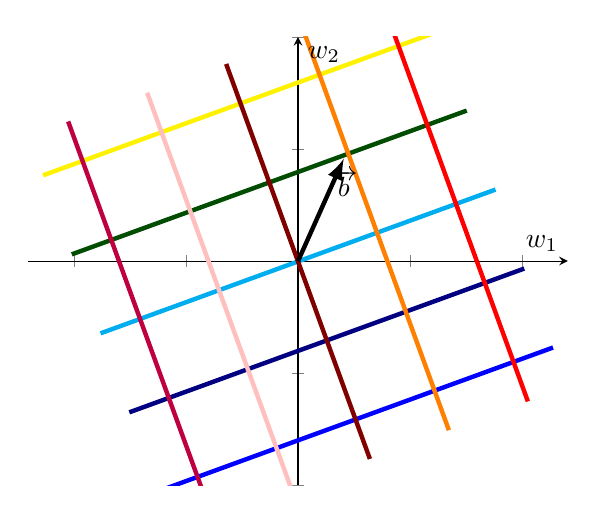
\begin{tikzpicture}
	\begin{axis}[
		axis lines=middle,
		axis equal,
		xmin=-4,
		xmax=4,
		ymin=-4,
		ymax=4,
		xlabel=$w_1$,
		ylabel=$w_2$,
		xticklabels={,,},
		yticklabels={,,}
	]
		\addplot[-, yellow, ultra thick, rotate=20, xshift= 0.8cm, yshift= -1.15cm] coordinates {(-3.75, 3) (3.75, 3)};
		\addplot[-, black!70!green, ultra thick, rotate=20, xshift= 0.8cm, yshift= -1.15cm] coordinates {(-3.75, 1.5) (3.75, 1.5)};
		\addplot[-, cyan, ultra thick, rotate=20, xshift= 0.8cm, yshift= -1.15cm] coordinates {(-3.75, 0) (3.75, 0)};
		\addplot[-, black!50!blue, ultra thick, rotate=20, xshift= 0.8cm, yshift= -1.15cm] coordinates {(-3.75, -1.5) (3.75, -1.5)};
		\addplot[-, blue, ultra thick, rotate=20, xshift= 0.8cm, yshift= -1.15cm] coordinates {(-3.75, -3) (3.75, -3)};
		
		\addplot[-, purple, ultra thick, rotate=20, xshift= 0.8cm, yshift= -1.15cm] coordinates {(-3, -3.75) (-3, 3.75)};
		\addplot[-, pink, ultra thick, rotate=20, xshift= 0.8cm, yshift= -1.15cm] coordinates {(-1.5, -3.75) (-1.5, 3.75)};
		\addplot[-, black!50!red, ultra thick, rotate=20, xshift= 0.8cm, yshift= -1.15cm] coordinates {(0, -3.75) (0, 3.75)};
		\addplot[-, orange, ultra thick, rotate=20, xshift= 0.8cm, yshift= -1.15cm] coordinates {(1.5, -3.75) (1.5, 3.75)};
		\addplot[-, red, ultra thick, rotate=20, xshift= 0.8cm, yshift= -1.15cm] coordinates {(3, -3.75) (3, 3.75)};
		
		\addplot[-latex, ultra thick] coordinates {(0, 0) ({2*cos(deg(20))}, {2*sin(deg(20))})} node[below] {$\overrightarrow{b}$};
	\end{axis}
\end{tikzpicture}